\newcommand{\thesistitle}{Integración de archivos y
 						  herramientas radioastronómicas 
						  en la arquitectura
						  del Observatorio Virtual}
\newcommand{\thesisauthor}{Juan de Dios Santander Vela}
\newcommand{\thesiskeywords}{}
\newcommand{\IAA}{Instituto de Astrofísica de Andalucía (CSIC)}
\newcommand{\fechaDeposito}{17 de Abril de 2009}

%Start by including hyperref and hypcap
\usepackage[
	pdftitle={\thesistitle},
	pdfauthor={\thesisauthor},
	pdfkeywords={\thesiskeywords}
	pdftex,
	bookmarksnumbered,
	colorlinks,
	backref,
	bookmarks,
	breaklinks,
	linktocpage
	]{hyperref}
% \usepackage[all]{hypcap}

%smalltabular es el estilo de todas las tablas pequeñas
\newenvironment{smalltabular}[1]
{\begin{center}
	\begin{small}
		\begin{tabular}{#1}}
{		\end{tabular}
	\end{small}
\end{center}}
\newenvironment{smallertabular}[1]
{\begin{center}
	\begin{footnotesize}
		\begin{tabular}{#1}}
{		\end{tabular}
	\end{footnotesize}
\end{center}}
\newenvironment{scriptsizetabular}[1]
{\begin{center}
	\begin{scriptsize}
		\begin{tabular}{#1}}
{		\end{tabular}
	\end{scriptsize}
\end{center}}

%minipage environment for tables: minitab
\newcommand{\minitab}[2][l]{\begin{tabular}{#1}#2\end{tabular}}

%Definición para obtener numeración simbólica de notas
\long\def\symbolfootnote[#1]#2{\begingroup%
\def\thefootnote{\fnsymbol{footnote}}\footnote[#1]{#2}\endgroup}

% Command to define dictionary-styled entries.
% First element is the word to be defined, second indicates the
% word kind (noun, verb, adverb, adjective...), and third is the
% actual definition. Uses the adjustwidth environment of the
% memoir class.

\newcommand{\dictionarydef}[3]{
	\begin{adjustwidth}{2\parindent}{\parindent}
			\textbf{#1}\\#2
			\begin{adjustwidth}{\parindent}{0cm}
				#3
			\end{adjustwidth}
	\end{adjustwidth}
}

\newcommand{\mtypedef}[4]{
	% #1 is the MType id
	% #2 is the MType description
	% #3 is a list of \mtypeparam entries
	% #4 is either none, or a list of \mtypeparam entries to return
%	\begin{minipage}{\columnwidth}
		\begin{adjustwidth}{\parindent}{\parindent}
			%\vspace{0.5cm}
			\textbf{#1}
			
			\begin{adjustwidth}{\parindent}{0pt}
				#2
				
				\begin{itemize}
					\item Arguments:
					
						\begin{itemize}
							#3
						\end{itemize}
						
					\item Return Values:
					
						\begin{itemize}
							#4
						\end{itemize}
						
				\end{itemize}
				
			\end{adjustwidth}

		\end{adjustwidth}
%	\end{minipage}
}

\newcommand{\mtypeparam}[4][]{
	% 1 is typically optional argument (typically, "optional")
	% 2 is the argument name
	% 3 is the argument type (for mtypes should be one of ...)
	% 4 is the argument description
	\def\optionalarg{#1}
	\def\emptyoption{}
	\ifx\optionalarg\emptyoption
		\def\nexttext{\item \texttt{#2} (#3): #4 }
	\else
		\def\nexttext{\item \texttt{#2} (#3) \emph{#1}: #4 }
	\fi \nexttext
}

\newcommand{\mtypeparamnone}[0]{\item none.}

% Concatenar cadenas:
\newcommand{\concatenate}[2]{#1#2}
\newcommand{\caltechbaseurl}[0]{http://viewcvs.cacr.caltech.edu}
\newcommand{\caltechpath}[0]{/us-vo/viewcvs.cgi/contrib/summerschool/}
\newcommand{\caltechsummerschool}[1]
{\concatenate{\concatenate{\caltechbaseurl}{\caltechpath}}{#1/}}
\newcommand{\caltechphpurl}[0]{\caltechsummerschool{php}}
\newcommand{\caltechpythonurl}[0]{\caltechsummerschool{python}}



% Prepare glossaryentry command for when glossary entries are
% to be prepared.
\newcommand{\glossaryentry}[1]{#1}


%urlnote is to create footnotes which contain URLs.
\newcommand{\urlnote}[1]{\footnote{\url{#1}}}

%Commands for URLs
\newcommand{\sesameurl}[0]
{http://cdsws.u-strasbg.fr/axis/services/Sesame?method=sesame&resultType=xi&name=M31}

\newcommand{\rainerirampubsurl}[0]
{http://adsabs.harvard.edu/cgi-bin/nph-abs_connect?library&libname=PV_Publ.&libid=45af8f27d3}

\newcommand{\irampakourl}[0]
{http://www.iram.es/IRAMES/documents/ncs30mPako/Current/PDF/pako.pdf}

\newcommand{\jsampurl}[0]
{http://deployer.astrogrid.org/software/jsamp/}

\newcommand{\sampyurl}[0]
{http://cosmos.iasf-milano.inaf.it/pandora/sampy.html}

\newcommand{\stiltsurl}[0]
{http://www.starlink.ac.uk/stilts/}


\newcommand{\massa}{\texttt{massa}}
\newcommand{\madcuba}{\texttt{madcuba}}



% invisiblenote: whatever is written inside does not get printed out
% by LaTeX; can be used for long comments; \invisible is added for
% differentiating between a long note and something that has turned
% to be invisible
\newcommand{\invisiblenote}[1]{}
\newcommand{\invisible}[1]{}
% supress is similar to Invisible, but can be used to provide
% who suggested the suppresion
\newcommand{\suppress}[2][]{} 

% visiblenote: whatever is written insided gets boxed
% and printed out
\newcommand{\boxednote}[1]{\begin{framed}{#1}\end{framed}}
\definecolor{shadecolor}{gray}{0.75}
\newcommand{\shadednote}[1]{\begin{shaded}{#1}\end{shaded}}
\newcommand{\leftbarnote}[1]{\begin{leftbar}{#1}\end{leftbar}}
\newcommand{\todo}[2][TO\-DO]{\leftbarnote{\noindent\textbf{#1}: #2}}
\newcommand{\todoblock}[1]{\begin{minipage}{\columnwidth}
\todo{#1}\end{minipage}}
\newcommand{\todoinline}[2][TO\-DO]{\fbox{\textbf{#1}: #2}}
\newcommand{\citeneeded}{\todoinline[needed]{cite/attribute}}
\newcommand{\lourdes}[1]{\todo[Lour\-des]{#1}}
\newcommand{\lourdesinline}[1]{\todoinline[Lour\-des]{#1}}
\newcommand{\todosuspended}[1]{}
\newcommand{\todoinlinesuspended}[1]{}
\newcommand{\todoblocksuspended}[1]{}

\newcommand{\ceil}[1]{\ensuremath{\lceil#1\rceil}}

\newcommand{\separator}[0]{
%\begin{adjustwidth}{0.33\textwidth}{0pt}
%	\rule{0.33\textwidth}{0.5pt}
%\end{adjustwidth}
\vfill
%	\begin{center}
%		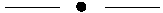
\includegraphics{fig/separator.pdf}
%	\end{center}
%\vfill
}

% Commands for semantic styling
\newcommand{\method}[1]{\texttt{#1}}
\newcommand{\mapkey}[1]{\texttt{#1}}
\newcommand{\datatype}[1]{\texttt{#1}}
\newcommand{\sampok}{\mapkey{samp.ok}}
\newcommand{\samperror}{\mapkey{samp.er\-ror}}
\newcommand{\sampwarning}{\mapkey{samp.warn\-ing}}
\newcommand{\sampresult}{\mapkey{samp.re\-sult}}
\newcommand{\sampstatus}{\mapkey{samp.sta\-tus}}
\newcommand{\sampmtype}{\mapkey{samp.mtype}}
\newcommand{\sampparams}{\mapkey{samp.pa\-rams}}
\newcommand{\stringtype}{\datatype{string}}
\newcommand{\listtype}{\datatype{list}}
\newcommand{\maptype}{\datatype{map}}
\newcommand{\sampint}{\datatype{SAMP int}}
\newcommand{\sampbool}{\datatype{SAMP bool\-e\-an}}
\newcommand{\sampfloat}{\datatype{SAMP float}}


% Commands/macros for VO protocol resumes
\def\semicolon{ semicolon (\texttt{;})}
\def\comma{ comma (\texttt{,})}
% \def\stringt{ \texttt{string} }
% \def\intt{ \texttt{integer} }
% \def\doublet{ \texttt{double} }

% Macros for XML tag and tags:

\newcommand{\xmlattr}[1]{\texttt{#1} at\-trib\-ute}
\newcommand{\xmlopen}[1]{\texttt{<#1>}}
\newcommand{\xmlclose}[1]{\texttt{</#1>}}
\newcommand{\xmlself}[1]{\texttt{<#1/>}}
\newcommand{\xmlenclose}[2]{
	\xmlopen{#1}\texttt{#2}\xmlclose{#1}
}
\newcommand{\xmlencloseattr}[3]{
	\xmlopen{#1 #2}\texttt{#3}\xmlclose{#1}
}
\newcommand{\xmltag}[1]{\xmlopen{#1} tag}
\newcommand{\xmltags}[1]{\xmlopen{#1} tags}
\newcommand{\dtdelement}[1]{\texttt{<!ELEMENT #1>}}
\newcommand{\dtdattlist}[1]{\texttt{<!ATTLIST #1>}}
\newcommand{\oxygenxml}[0]{
	Generated with the XML Schema diagram generator of the oXygen XML
	Editor.
}

\newenvironment{attributedquotenv}{
	\epigraphposition{flushright}
	\epigraphtextposition{flushleftright}
	\epigraphsourceposition{flushright}
	\setlength{\epigraphwidth}{0.6\textwidth}
	\setlength{\parindent}{1em}
}

\newcommand{\attributedquote}[2]{
	\begin{attributedquotenv}
		\epigraph{#1\hspace*{\fill}}{\emph{#2}\hspace*{\fill}}
	\end{attributedquotenv}
}
% The \hspace*{\fill} parts are needed in order to avoid
% the 

%Superscript and subscript commands, with common endings
%\newcommand{\superscript}[1]{\ensuremath{^{\textrm{#1}}}}
%\newcommand{\textsubscript}[1]{\ensuremath{_{\textrm{#1}}}}
\newcommand{\thsup}[0]{\textsuperscript{th}}
\newcommand{\stsup}[0]{\textsuperscript{st}}
\newcommand{\ndsup}[0]{\textsuperscript{nd}}
\newcommand{\rdsup}[0]{\textsuperscript{rd}}

\newcommand{\water}{\ensuremath{\textrm{H}_2\textrm{O}}}

%\newcommand{\classname}[1]{\fontencoding{OT1}\fontfamily{cmss}\fontseries{m}\fontshape{n}\fontsize{12}{15}\selectfont#1\normalfont}
%\newcommand{\classname}[1]{\textsf{#1}}
\newcommand{\classname}[1]{#1}

\newcommand{\ttmath}[1]{$\mathtt{#1}$}
\newcommand{\ucd}[1]{\texttt{UCD}$\mathtt{=}$\texttt{#1}}
\newcommand{\ttequals}[2]{\texttt{#1}\texttt{=}\texttt{#2}}

% Listings: Renew command \lstlistlistingname to change name into Spanish
\renewcommand{\lstlistlistingname}{Índice de listados}
\lstset{
	basicstyle=\tiny\ttfamily
}

% Hyphenation commands
\hyphenation{da-ta-base}
\hyphenation{da-ta-ba-ses}
\hyphenation{ex-tra-ga-lac-tic}
